\documentclass[conference]{IEEEtran}
\IEEEoverridecommandlockouts
% The preceding line is only needed to identify funding in the first footnote. If that is unneeded, please comment it out.
\usepackage{cite}
\usepackage{amsmath,amssymb,amsfonts}
\usepackage{algorithmic}
\usepackage{graphicx}
\usepackage{textcomp}
\usepackage{xcolor}
\usepackage{tabularx}
\usepackage{multirow}
\usepackage{graphics} % for pdf, bitmapped graphics files
\usepackage{subfig}
\usepackage{subcaption}
\usepackage{hyperref}
\usepackage{academicons}
\usepackage{xcolor}
\usepackage{listings}
\def\BibTeX{{\rm B\kern-.05em{\sc i\kern-.025em b}\kern-.08em
		T\kern-.1667em\lower.7ex\hbox{E}\kern-.125emX}}
% Gráficas en MATLAB
\usepackage{tikz, pgfplots}
% Color Enlace
\definecolor{colorEnlace}{RGB}{0, 0, 0}
\hypersetup{
	colorlinks=true,
	linkcolor=colorEnlace,
	citecolor=colorEnlace,
	urlcolor=colorEnlace,
	pdfauthor={Ruth Juana Espino Puma, Davis Bremdow Salazar Roa},
	pdftitle={}
}
% Control 
\usepackage{amsmath}
\begin{document}
	
	\title{Experiencia N°4 - Diseño de Controlador PID}
	
	\author{
		\IEEEauthorblockN{Ing. Darcy Arredondo Huarac}
		\IEEEauthorblockA{
			Laboratorio de Control I\\
			Cusco, Perú\\
			diego.arredondo@unsaac.edu.pe}
		\and
		\IEEEauthorblockN{Ruth Juana Espino Puma}
		\IEEEauthorblockA{
			Estudiante de Ingeniería Electrónica \\
			Cusco, Perú \\
			184657@unsaac.edu.pe}
		\and
		\IEEEauthorblockN{Davis Bremdow Salazar Roa}
		\IEEEauthorblockA{
			Estudiante de Ingeniería Electrónica \\
			Cusco, Perú \\
			200353@unsaac.edu.pe
		}
	}
	
	\maketitle
	\begin{abstract}
		The document outlines the design of a PID controller using the Ziegler-Nichols tuning method for an analog control system. The objectives include designing controllers for underdamped and overdamped cases, aiming to reduce overshoot and response time. For the underdamped case, calculations for parameters \( k_p \), \( k_i \), and \( k_d \) are based on a derived transfer function, with the system tuned to cut overshoot by half. For the overdamped case, similar calculations optimize response time. Simulations in MATLAB/Simulink demonstrate step and impulse responses, highlighting improvements in control. Additionally, the document presents PID circuit designs with specified resistor and capacitor values for each damping case, along with simulated output graphs for analysis.
	\end{abstract}
	
	\begin{IEEEkeywords}
		PID controller design, Ziegler-Nichols method, analog control system, underdamped response, overdamped response, transfer function, gain tuning, MATLAB/Simulink simulation, circuit design, response optimization
	\end{IEEEkeywords}
	\section{\textbf{Informe Final}}
	\subsection{\textbf{Muestre las gráficas obtenidas con el Osciloscopio para el caso Subamortiguado y Sobreamortiguado en lazo cerrado}}
	
	\begin{figure}[h]
		\centering
		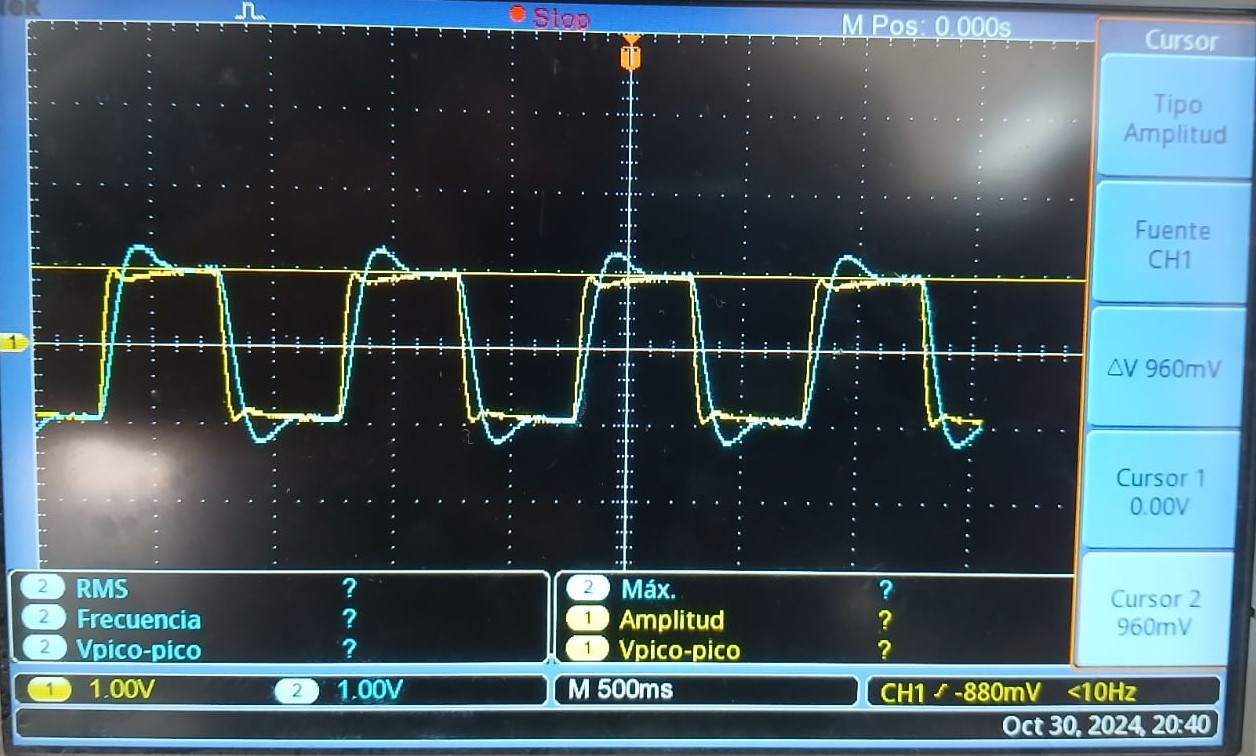
\includegraphics[width=0.4\textwidth]{media/sub-respuesta-general.jpeg}
		\caption{Comparación de la respuesta del sistemas - PID}
		\label{fig:sub-respuesta-general}
	\end{figure}
	
	\begin{figure}[h]
		\centering
		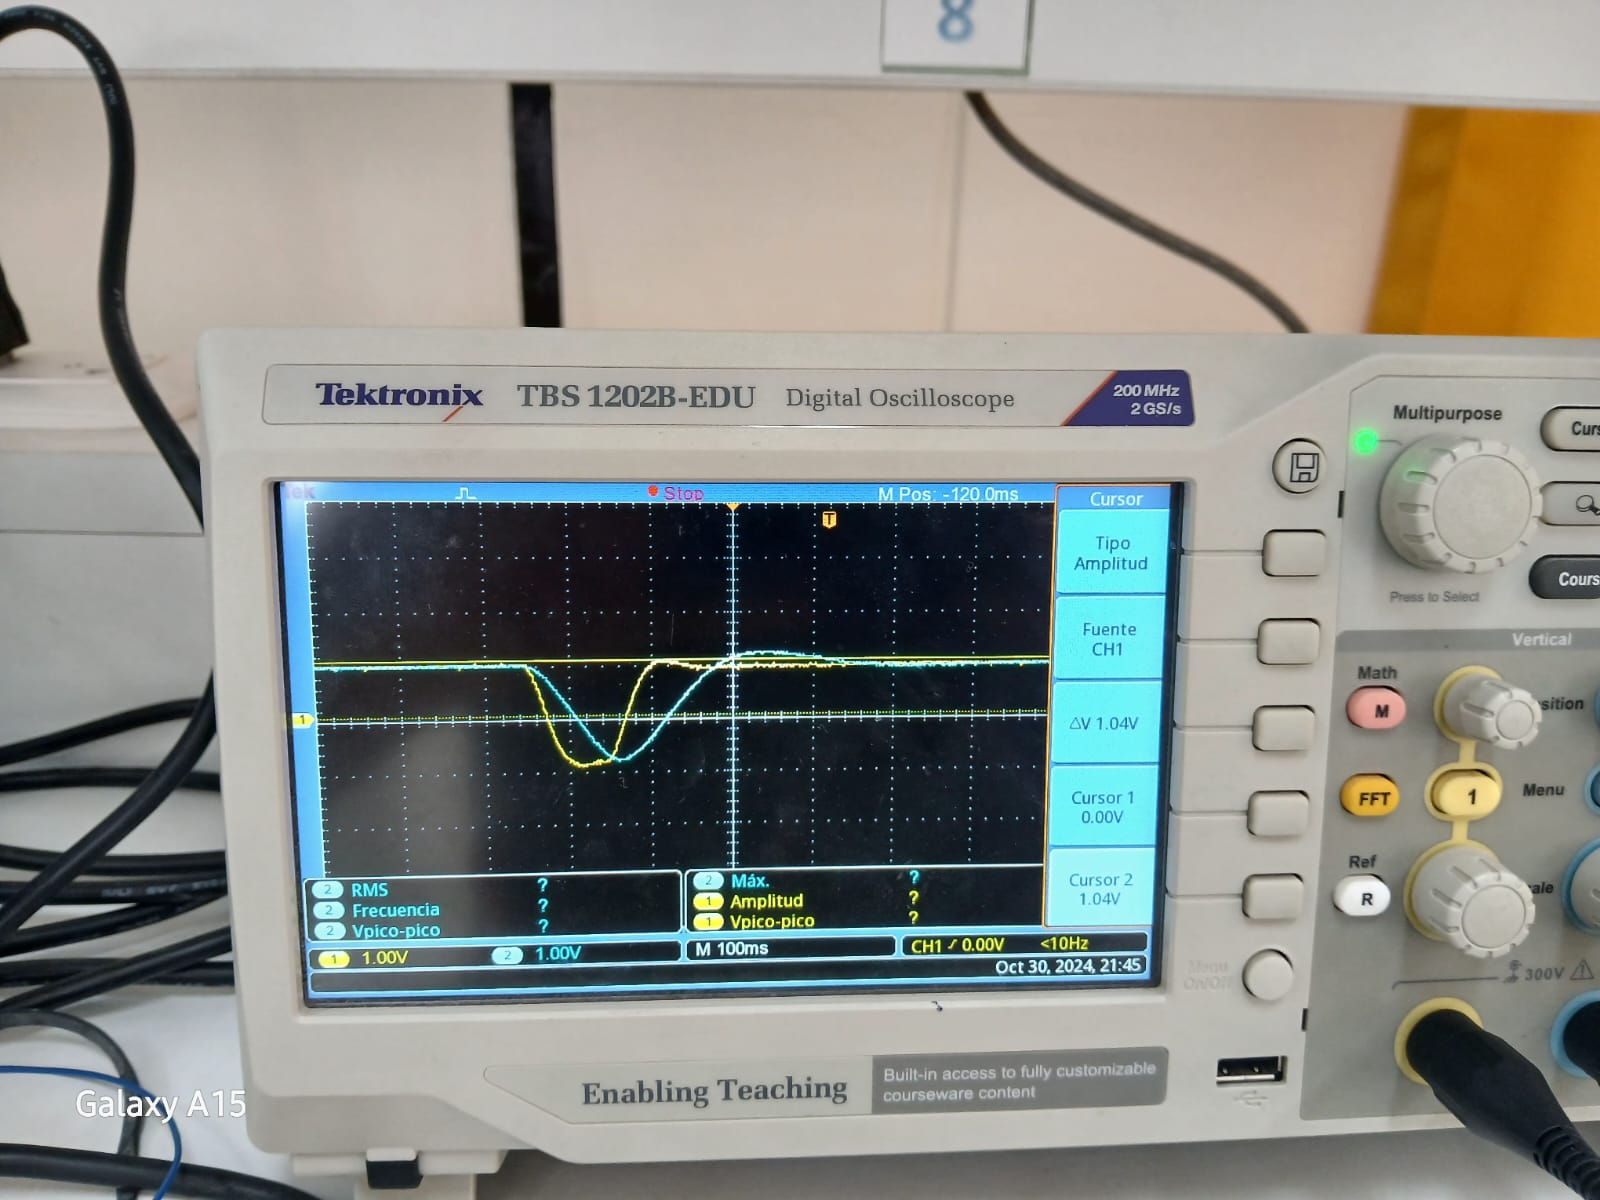
\includegraphics[width=0.4\textwidth]{media/sub-sobrepico-104.jpeg}
		\caption{Sobrepico del sistema subamortiguado - PID}
		\label{fig:sub-sobrepico-104}
	\end{figure}
	
	\begin{figure}[h]
		\centering
		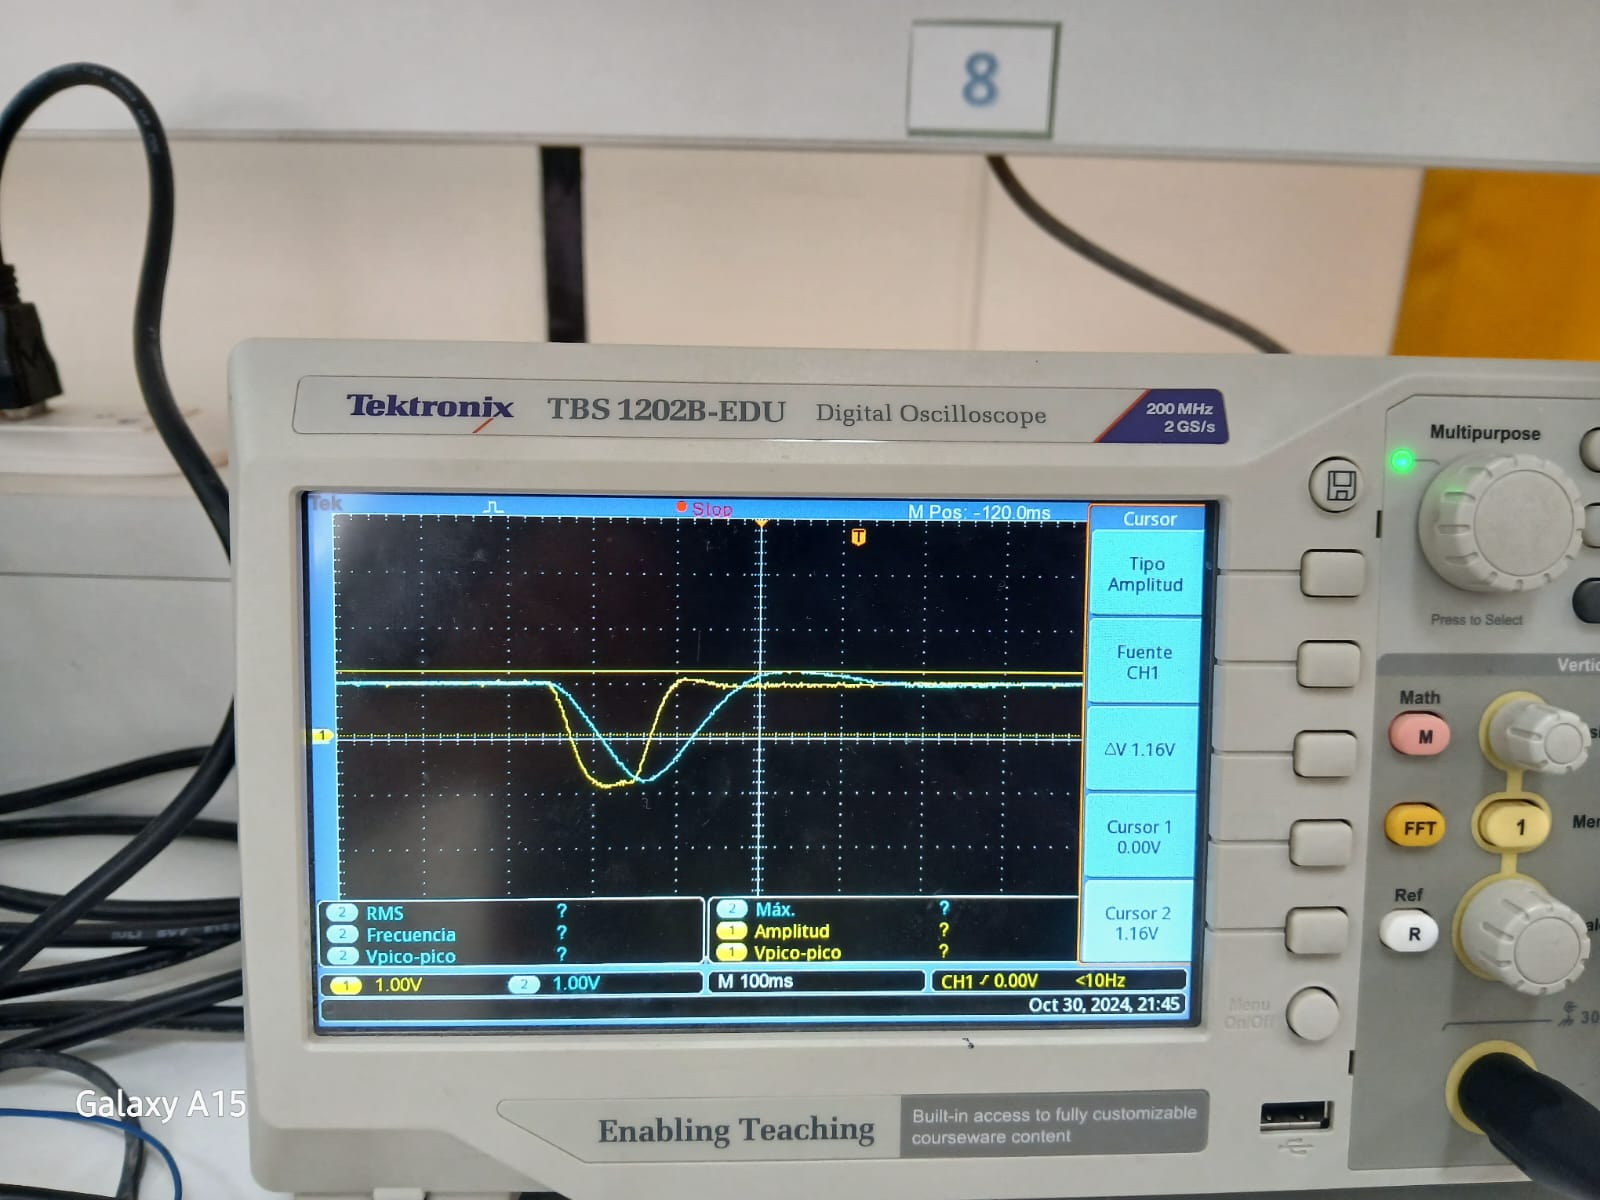
\includegraphics[width=0.4\textwidth]{media/sub-sobrepico-116}
		\caption{Sobrepico del sistema subamortiguado sin PID}
		\label{fig:sub-sobrepico-116}
	\end{figure}
		
	\subsection{\textbf{¿La respuesta hallada en forma teórica es igual o similar al circuito implementado?}}
	
	Para realizar la comparación entre las respuestas del sistema será necesario definir de forma precisa la relación que se tiene entre las diferentes entradas para el circuito
	
	En la figura \ref{fig:sub-sobrepico-simulado} se puede apreciar la respuesta del sistema frente a una señal cuadrada siendo la señal de color verde la respuesta sin la compensación mediante PID y la naranja la señal de respuesta con el sobrepico disminuido al aplicar el control PID a la planta.
	\begin{figure}[h]
		\centering
		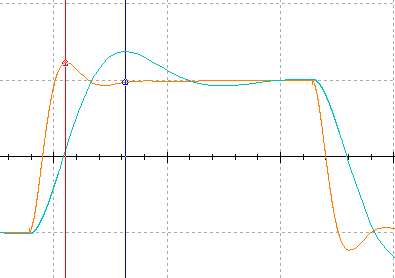
\includegraphics[width=0.5\textwidth]{media/sub-sobrepico-simulado}
		\caption{Respuesta del sistema subamortiguado en Multisim}
		\label{fig:sub-sobrepico-simulado}
	\end{figure}
	
	
	
	\subsection{\textbf{Comente acerca del error de la señal de salida con respecto a la señal de entrada}}
	
	\section{Conclusiones}
	
	\bibliographystyle{IEEEtran}
	\bibliography{biblio}
\end{document}